\chapter{LITERATURE REVIEW}
\label{chap-two}
Bridges are designed based on discrete events with minimal consideration of interactions between hazards/loading, material aging (or more accurately condition) and bridge performance. The purpose of the research described is to study Time Dependent Performance Based Design that considers the effects of cumulative damage on the properties of the materials.

In this chapter the available knowledge on the different topics that are available in the literature are summarized. First a review on the different definitions of commutative damage is presented then the main idea for this research are established and the required components, then the different elements that form part of this study are presented and  a general concept is established and presented in Chapter 3.

\section{Cumulative Damage}

There have been attempts by many researchers to stablish the best way to account for the accumulation of damage. 

\subsection{Damage Index}
The effect of commulative damage in structures was first studied by by Park and Ang (1985) \cite{Young-JiPark1985} in their study the authors proposed an expresion that intended to quantify damage in a structure and on the basis of it classify the extent of damage to recommend wether a structure could be used or not. This expresion was coined as the Damage Index ($D$) and it is exprssed as follows:

\begin{equation}
  D=\frac{\Delta_{m}}{\Delta_{u}}-\beta \frac{E_h}{F_{y}\Delta{u}}
  \label{eq.DamageIndex}
\end{equation} 

$Delta_{m}$: Maximum deformation under earthquake

$Delta_{u}$: Ultimate deformation under monotonic loading

$F_{y}$: Calculated yield strength

$E_{h}$: Total hysteretic energy

$\beta$: Dimensionless constant 

\begin{figure}[htbp]
\centering
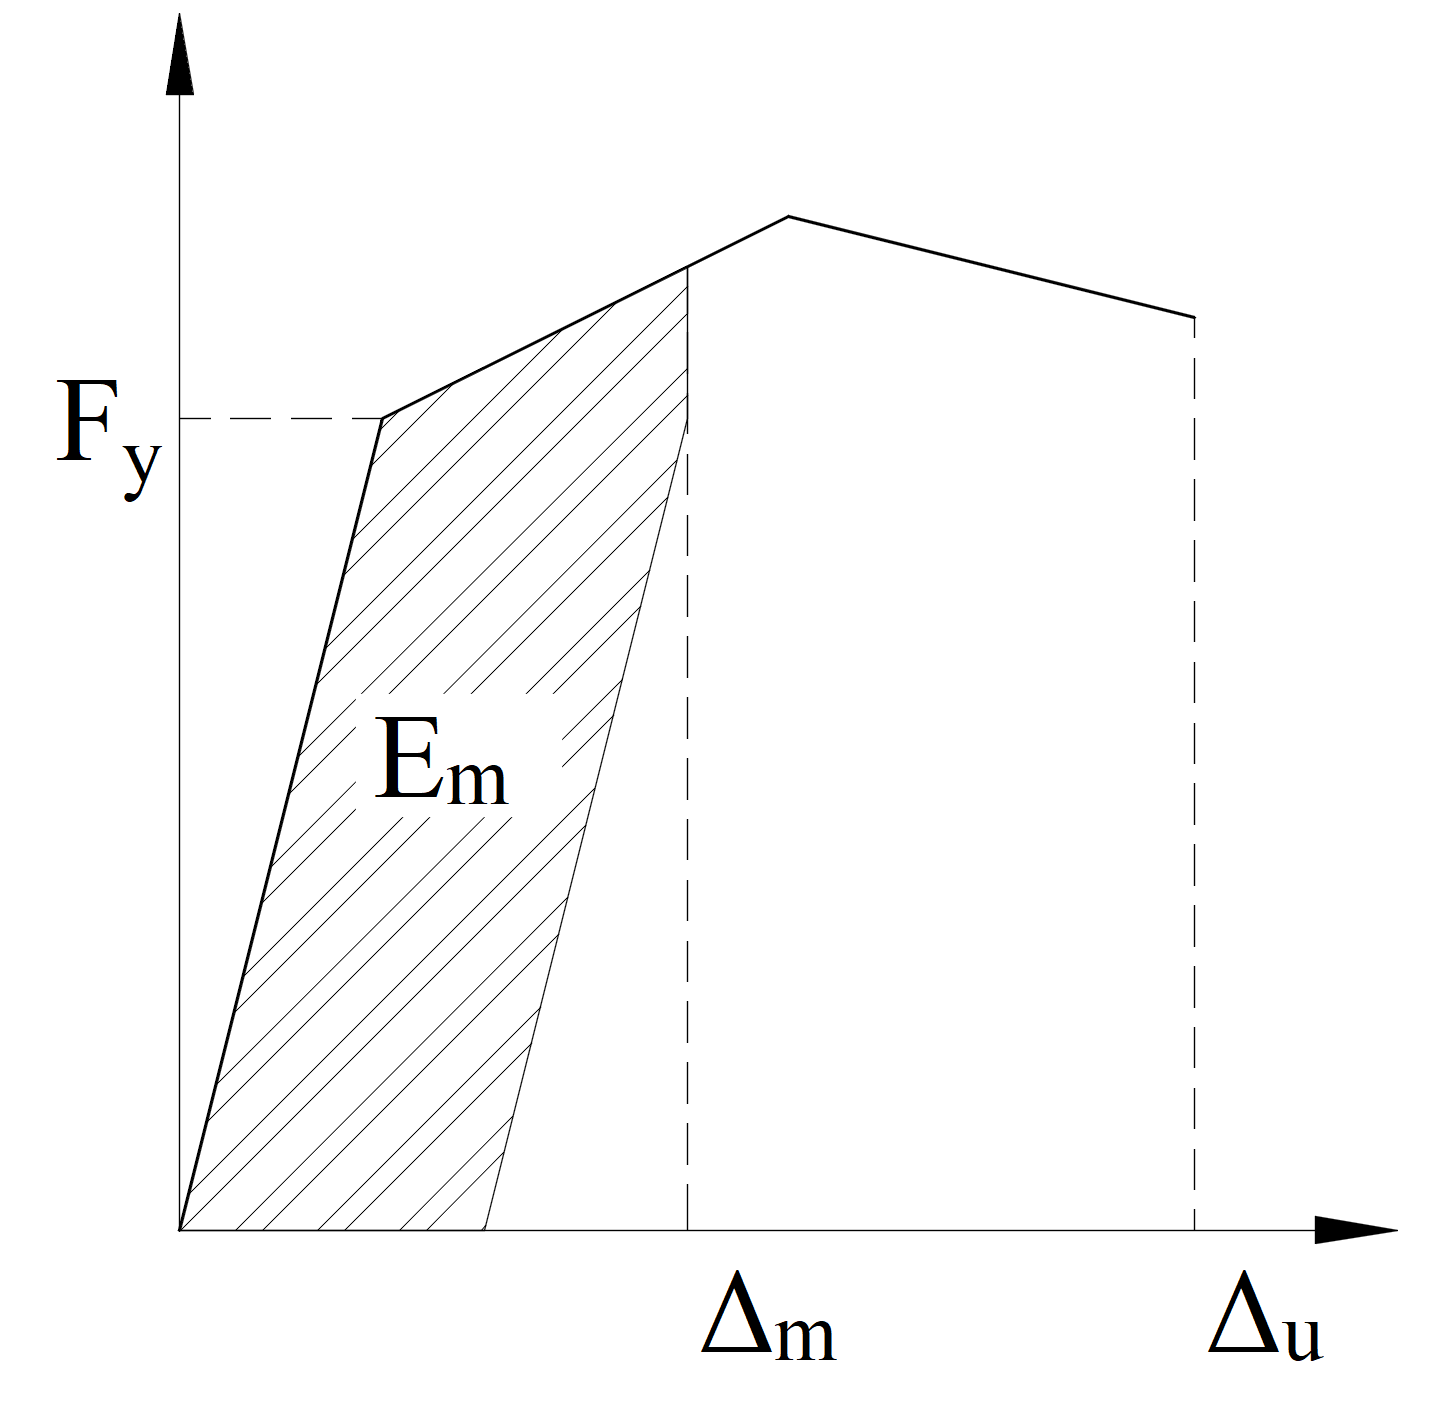
\includegraphics[width=0.9\textwidth]{Chapter-2/figs/Park_and_Ang_Model}
\caption{Parkn and Ang conceptual scheme}
\label{fig:Paa}
\end{figure}

This equation was derived for concrete elements. The first term here is a simple, pseudo-static displacement measure. It takes no account of cumulative damage, which is accounted for solely by the energy term. A figure on the concept is shown in \fref{fig:Paa}. The advantages of this model are its simplicity, and the fact that it has been calibrated against a significant amount of observed seismic damage, included some instances of shear and bond failures. Park, Ang and Wen (1985) suggested D = 0.4 as a threshold value between repairable and irreparable damage. 

One of the disadvantages of this model is the need to calibrate the $\beta$ coefficient with observed damage, this value is typically a very low coefficient $\beta=0.05-0.1$ rendering the second term relatively inconsequential. 

Several studies have used or modified this model to study the effects of cumulative damage for different structures,  of relevant importance are those performed by \cite{Kunnath1992}, who used a modified Park and Ang model, to model damagae at the local level for elements in a structural analysis program IDARC 3.0, in this software for the case of multiple degrees of freedom buildings they also added parameters to consider the damage at the inter-story level and the global model. Other studies \cite{Khashaee} have proposed an damage index that has a strong correlation with the portion of the earthquake energy that is associated with inelastic action, they used this damage index to perform a damage based design. While this studies provide insight into some of the characteristics of damage accumulation they rely on the Park and Ang model and therefore carry the issue of having a very low $\beta$ coefficient and thus the nonlinear portion of the structure is not considered.

Krawinkler (1987) \cite{Krawinkler1987} proposed a method that would consider damage as a function of low cycle fatigue parameters, the form of this damage index for Steel Component, Weldements and local buckling have a general shape of the Miner model. This model relies on the accumulation of plastic deformations. While this model has proven to work well for the evaluation of individual elements it does not provide a way to generalize damage for other types of structures.

\subsection{Fragility Curves}

